\documentclass{VUMIFPSkursinis}
\usepackage{algorithmicx}
\usepackage{algorithm}
\usepackage{algpseudocode}
\usepackage{amsfonts}
\usepackage{amsmath}
\usepackage{bm}
\usepackage{caption}
\usepackage{color}
\usepackage{float}
\usepackage{graphicx}
\usepackage{listings}
\usepackage{subfig}
\usepackage{wrapfig}

\usepackage{enumitem}
%PAKEISTA, tarpai tarp sąrašo elementų
\setitemize{noitemsep,topsep=0pt,parsep=0pt,partopsep=0pt}
\setenumerate{noitemsep,topsep=0pt,parsep=0pt,partopsep=0pt}

% Titulinio aprašas
\university{Vilniaus universitetas}
\faculty{Matematikos ir informatikos fakultetas}
\department{Programų sistemų katedra}
\papertype{Programų sistemų inžinerijos I laboratorinis darbas}
\title{Socialinis Vilniaus universiteto tinklalapis}
\titleineng{SocialVU}
\status{2 kurso 4 grupės studentai}
\author{Andrejus Voitovas}
\secondauthor{Eglė Puodžiūnaitė}
\thirdauthor{Kasparas Kralikas}
\fourthauthor{Ieva Vizgirdaitė} % Pridėti antrą autorių
\supervisor{asist. dr. Vytautas Valaitis}
\date{Vilnius – \the\year}

% Nustatymai
% \setmainfont{Palemonas}   % Pakeisti teksto šriftą į Palemonas (turi būti įdiegtas sistemoje)
\bibliography{bibliografija}

\begin{document}
	
% PAKEISTA	
\maketitle
\cleardoublepage\pagenumbering{arabic}
\setcounter{page}{2}

%TURINYS
\tableofcontents

\sectionnonum{Įvadas}
Tikslas - sukurti socialinio tinklalalapio prototipą, kurį įgyvendinus būtų palengvinta universiteto bendruomenės komunikaciją.

Temos aktualumas:
Šiuo metu studentams dėstytojų skelbiama informacija yra išbarstyta internete, kurią surasti užima galybes laiko. Yra atskiras universiteto naujienų puslapis, kiekvienas dėstytojas turi savo asmeninį tinklalapį, atskiras elektroninis paštas. Tiek dėstytojui pasiekti studentus, tiek studentui dėstytoją yra komplikuota ir nepatogu.

Siekiami rezultatai:

\sectionnonum{VERSLO PROCESO APRAŠAS}
\section{IŠORINĖ VERSLO PROCESO ANALIZĖ}
Išorinė analizės metu išsiaiškinami ištekliai
reikalingi pradėti verslą, išryškinamos kuriamo verslo grėsmės ir
problemos, kuriami tinklalapio teikiami rezultatai ir išanalizuojama rinkoje esanti situacija. Nustačius rinkoje esančius ir potencialius konkurentus išanalizuojamos
neišnaudotos galimybės bei įvertinama situacija.

1, 2, 3 ir 4 lentelėse pateikiami įeigos, išeigos, reguliavimo ir įvaizdžio svarbiausi vertinimo kriteriai,
jų matavimo vienetai. Nustatoma kritinė vertė, esama vertė ir siekiama vertė. Tai padeda
nustatyti, ar tam tikras vertinimo kriterijus atitinka normas.
\subsection{Įeigos}
\begin{enumerate}
	\item Studentai
	\item Dėstytojai
	\item Administratorius
	\item Duomenų bazė
	\item Serveris
\end{enumerate}
\begin{table}[H]\footnotesize
	\centering
	\caption{Įeigos}
	\resizebox{\textwidth}{!}{\begin{tabular}{|c|c|c|c|} \hline
			Vertinimo kriterijus & Mertinimo matas & Siekiama vertė & Kritinė vertė \\
			\hline
			Studentai & Kiekis studentų, naudojančių socialVU tinklalapį & 21281 & 10000 \\
			\hline
			Dėstytojai & Kiekis dėstytojų, naudojančių socialVU tinklalapį & 2890 & 1500 \\
			\hline
			Administratorius & Pašalintų naudotojų skaičius per
			mėnesį & 0 & 30 \\
			\hline
			Duomenų bazė & Talpa GB & 50 & 10 \\
			\hline
			Serveris & Vidutinis užklausos apdorojimo laikas sekundėmis & 1 & 5 \\
			\hline
	\end{tabular}}
\end{table}
\subsection{Išeigos}
\begin{enumerate}
	\item Studentai, radę visą reikiamą informaciją
	\item Dėstytojai, pateikę visą norimą informaciją
\end{enumerate}
\begin{table}[H]\footnotesize
	\centering
	\caption{Išeigos}
	\resizebox{\textwidth}{!}{\begin{tabular}{|c|c|c|c|} \hline
			Vertinimo kriterijus & Mertinimo matas & Siekiama vertė & Kritinė vertė \\
			\hline
			Studentai, radę visą reikiamą informaciją & Kiekis per mėnesį \% & 100 & 50 \\
			\hline
			Dėstytojai, pateikę visą norimą informaciją & Kiekis per mėnesį \% & 100 & 50 \\
			\hline
	\end{tabular}}
\end{table}
	\subsection{Įvaizdis}
\begin{enumerate}
	\item Dėstytojų bei studentų atsiliepimai
	\item Sistemos žinomumas
\end{enumerate}
\begin{table}[H]\footnotesize
	\centering
	\caption{Įvaizdis}
	\resizebox{\textwidth}{!}{\begin{tabular}{|c|c|c|c|} \hline	
			Vertinimo kriterijus & Mertinimo matas & Siekiama vertė & Kritinė vertė \\
			\hline
			Dėstytojų bei studentų atsiliepimai & Teigiamų atsiliepimų \% nuo visų atsiliepimų & 90 & 50 \\
			\hline
			Sistemos žinomumas & Vilniaus universiteto studentų \% žinančių šį tinklalapį & 100 & 50 \\
			\hline
	\end{tabular}}
\end{table}
	\subsection{Reguliavimas}
\begin{enumerate}
	\item Asmens duomenų teisinės apsaugos įstatymas
	\item Darbo kodeksas
\end{enumerate}
\begin{table}[H]\footnotesize
	\centering
	\caption{Įvaizdis}
	\resizebox{\textwidth}{!}{\begin{tabular}{|c|c|c|c|} \hline
			Vertinimo kriterijus & Mertinimo matas & Siekiama vertė & Kritinė vertė \\
			\hline
			Asmens duomenų teisinės apsaugos įstatymas & Pažeidimų skaičius & 0 & 0 \\
			\hline
			Darbo kodeksas & Viršytas darbo laikas (kartais per metus) & 0 & 0 \\
			\hline
	\end{tabular}}
\end{table}
\subsection{Grėsmės}
Kuriamas verslas yra priklausomas nuo dviejų pagrindinių įvesčių - dėstytojų ir studentų. Jų skaičius ir aktyvumas lemia kuriamos programos sėkmę. Rinkoje jau egzistuoja nemažai socialinių tinklų, kuriuos naudoja dauguma studentų (Facebook, Instagram, Linkedin, Twitter ir t.t.) be to dauguma dėstytojų yra ipratę skelbti visą informaciją savo sukurtuose puslapiuose arba bando integruoti informaciją į Vilniaus universiteto virtualią mokymosi aplinką, todėl konkurencija yra gana didelė. Kuo daugiau dėstytojų pradės naudoti mūsų sukurtą platformą, tuo daugiau studentų taip pat privalės naudoti šį tinklalapį, nes tik ten galės rasti jiems reikiamą informaciją. Sėkmingam kuriamo verslo proceso egzistavimui turi įtakos reitingų ir atsiliepimų skaičius bei kokybė, tačiau visų pirma reikia užtikrinti, jog dauguma studentų bei dėstytojų išbandytų mūsų sukurtą sistemą bei ją įvertintų.
\subsection{Neišnaudotos galimybės}
Rinkoje jau egzistuojančios Vilniaus universiteto platformos turi trūkumų (dauguma dėstytojų skelbia informaciją skirtinguose puslapiuose, todėl studentams sunku juos surasti, ne visada yra galimybė susisiekti su dėstytojais, dauguma konspektų nėra lengvai pasiekiami visiems studentams), todėl kuriama sistema gali juos išnaudoti ir pasiūlyti studentams visą reikiamą informaciją rasti vienoje vietoje. Sistema suteiks galimybę išsiųsti laišką dėstytojui bei rasti visą paskelbtą dėstytojo informaciją vienoje vietoje, studentai galės matyti naujausią informaciją bei terminus iki kada turi atlikti tam tikras užduotis. Be to vienoje vietoje galės rasti visus reikiamus konpektus bei pasidalinti turimais konspektais su kitais studentais ir taip padėti mokytis kitiems.
\section{VIDINĖ VERSLO PROCESO ANALIZĖ}
Toliau pateikiama keliais aspektais atlikta vidinė verslo proceso analizė, kuria siekiama
nustatyti nagrinėjamo verslo stiprybes ir silpnybes, kylančias iš verslo proceso.
\subsection{Dalykinės srities statinė stukrtūra}
 Toliau pateikiama dalykinės srities statinės struktūros UML diagrama. Joje matomos pag-
rindinės esybės bei jų tarpusavio sąveika. Klientai yra dviejų tipų: studentai, dėstytojai ir administratoriai (dėstytojai bei administratoriai skiriasi turinio redagavimo teisėmis). Studentams, administratoriams ir dėstytojams registruotis nereikia, nes visa vartotojų duomenų bazė bus imama iš bendros VU vartotojų duomenų bazės. Vartotojui tereikia autentifikuoti save - tokiu būdu, priklausomai nuo užimamų pareigų, jam bus suteiktos teisės prie numatyto turinio. Studentai gali tik skaityti tokius puslapius kaip "Dėstytojai", "Naujienos", "Renginiai", "D.U.K". Tuo tarpu dėstytojai skiltyje "Naujienos" gali parašyti naujieną. Be to, jiems suteikta prieiga prie jų profilio, kur turi teisę redaguoti savo asmeninį puslapį pagal mūsų sukurtą šabloną, siųsti bei gauti žinutes, pridėti organizuojamą renginį. Administratoriumi gali būti fakulteto paskirtas žmogus, atsakingas už tikslingo turinio formavimą vidiniame socialiniame tinkle arba VU Studento atstovybės narys, kuris turi teisę redaguoti visą turinį. Tačiau joks administratorius negali redaguoti dėstytojo sukurto turinio, nes taip numato mūsų kurtas produktas.\\

SĄVOKOS: \\
Šiame skyriuje pateikiami specifiniai mūsų projekte naudotų žodžių paaiškinimai. \\
\textbf{Sistema} – fakulteto vidinis socialinis tinklas, dokumente vadinamas „SocialVU“. \\
\textbf{Studentas} – vartotojas, kuris turim ribotas galimybes turinio valdymo atžvilgiu.\\
\textbf{Dėstytojas} – vartotojas, kuris turi galimybę redaguoti visą socialinio tinklo turinį.\\
\textbf{Administratorius} – vartotojas, kuris turi galimybę redaguoti visą socialinio tinklo turinį, išskyrus dėstytojus.

\subsection{Užduotys}
\setlength{\parindent}{0pt}\textbf{Užduotis:} sukurti naujieną. \\
\textbf{Tikslas:} publikuoti naujieną, kuri būtų įdomi.\\
\textbf{Trigeris:} administratoriaus arba dėstytojo kuriama naujiena tituliniui. \\
\textbf{Prioritetas:} aukštas. \\
\textbf{„Prieš” sąlygos:} naujiena bus skaitoma.\\
\textbf{Sėkmingos baigties „po” sąlyga:} naujiena perskaitoma ir įsisavinama nauja informacija. \\
\textbf{Nesėkmingos baigties sąlyga:} naujiena visiškai nėra skaitoma. \\
\textbf{Pirminis agentas:} administratorius. \\
\textbf{Antriniai agentai:} studentas. \\ 

\setlength{\parindent}{0pt}\textbf{Užduotis:} redaguoti puslapį. \\
\textbf{Tikslas:} redaguoti dėstytojo puslapį.\\
\textbf{Trigeris:} prisijungęs dėstytojas gali redaguoti puslapį. \\
\textbf{Prioritetas:} aukštas. \\
\textbf{„Prieš” sąlygos:} dėstytojas patogiai talpina informaciją.\\
\textbf{Sėkmingos baigties „po” sąlyga:} dėstytojo informacija sudėliota pagal šabloną ir patogi naudojimuisi. \\
\textbf{Nesėkmingos baigties sąlyga:} dėstytojas nesudaro savo puslapio. \\
\textbf{Pirminis agentas:} dėstytojas. \\
\textbf{Antriniai agentai:} studentas. \\

\setlength{\parindent}{0pt}\textbf{Užduotis:} sukurti renginį. \\
\textbf{Tikslas:} publikuoti renginį, kuris būtų naudingas.\\
\textbf{Trigeris:} administratoriaus arba dėstytojo sukurtas renginys atsiranda puslapyje. \\
\textbf{Prioritetas:} aukštas. \\
\textbf{„Prieš” sąlygos:} renginį aplankys daug žmonių.\\
\textbf{Sėkmingos baigties „po” sąlyga:} renginys pateisino savo lūkesčius. \\
\textbf{Nesėkmingos baigties sąlyga:} apie renginį studentai sužinojo ne iš socialinio tinklo. \\
\textbf{Pirminis agentas:} administratorius. \\
\textbf{Antriniai agentai:} studentas. \\


\setlength{\parindent}{0pt}\textbf{Užduotis:} parašyti žinutę. \\
\textbf{Tikslas:} parašyti žinutę tiesiai vartotojui.\\
\textbf{Trigeris:} studentas, paspaudęs ant dėstytojo, gali parašyti jam žinutę. \\
\textbf{Prioritetas:} aukštas. \\
\textbf{„Prieš” sąlygos:} vartotojas gaus žinutę.\\
\textbf{Sėkmingos baigties „po” sąlyga:} vartotojai patogiai komunikuos tarpusavy. \\
\textbf{Nesėkmingos baigties sąlyga:} žinutė liks neperskaityta. \\
\textbf{Pirminis agentas:} studentas. \\
\textbf{Antriniai agentai:} administratorius.\\

\setlength{\parindent}{0pt} \textbf{Užduotis:} apsilankyti asmeniniame puslapyje. \\
\textbf{Tikslas:} pasiekti dėsytotojo asmeninį puslapį.\\
\textbf{Trigeris:} studentų apsilankymas dėstytojų profilyje. \\
\textbf{Prioritetas:} aukštas. \\
\textbf{„Prieš” sąlygos:} vartotojai lankysis dėstytojų puslapiuose per socialinį tinklą.\\
\textbf{Sėkmingos baigties „po” sąlyga:} vartotojams bus patogu pasiekti puslapį ir sužinoti informaciją. \\
\textbf{Nesėkmingos baigties sąlyga:} vartotojai toliau ieškos puslapių naudojantis "Google". \\
\textbf{Pirminis agentas:} studentas. \\
\textbf{Antriniai agentai:} administratorius.

\subsection{Užduočių vykdymo scenarijai}
\ref{fig:klasiu} pav. paveikslėlyje pavaizduota esybių diagrama. Pateikiamos pagrindinės dalykinės srities esybės, pavaizduoti ryšiai tarp jų. 
\begin{figure}[H]
\centering
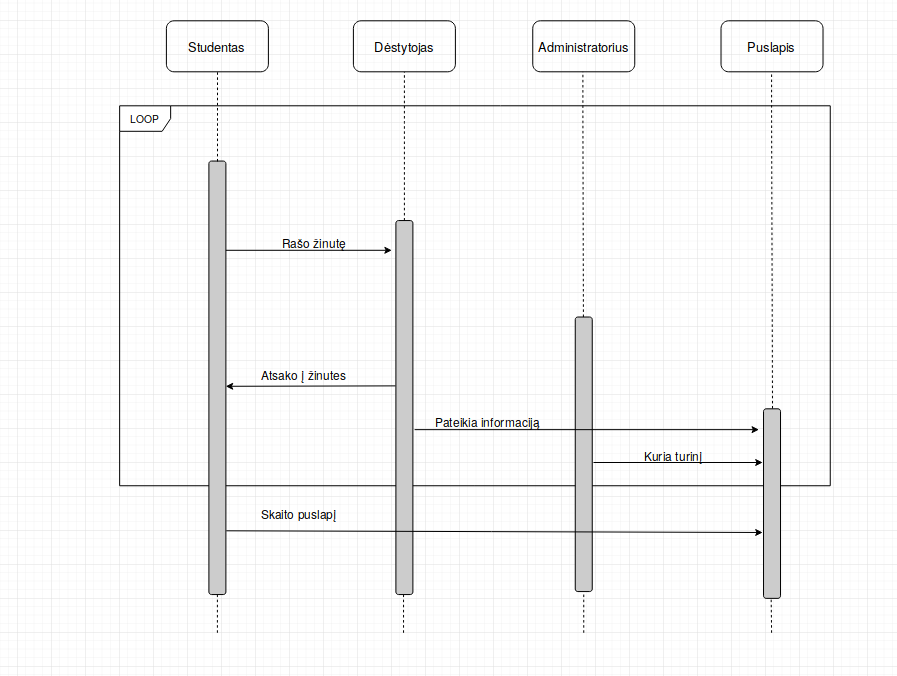
\includegraphics[width=\linewidth]{img/bendra-uml.png}
\caption{Klasių diagrama}
\label{fig:klasiu}
\end{figure}
1 pav. vaizuduojamas socialinio tinklo naudojimosi modelis. Studentas gali rašyti dėstytojui žinutę, o dėstytojas jam gali atsakyti. Taip pat studentas skaito puslapį, kurį pats dėstytojas ir sukūrė. Administratorius kuria turinį, į kurį įeina: renginiai, naujienos, D.U.K.
\subsection{Dalykinės srities dinaminė struktūra}
Studentas:
\begin{figure}[H]
\centering
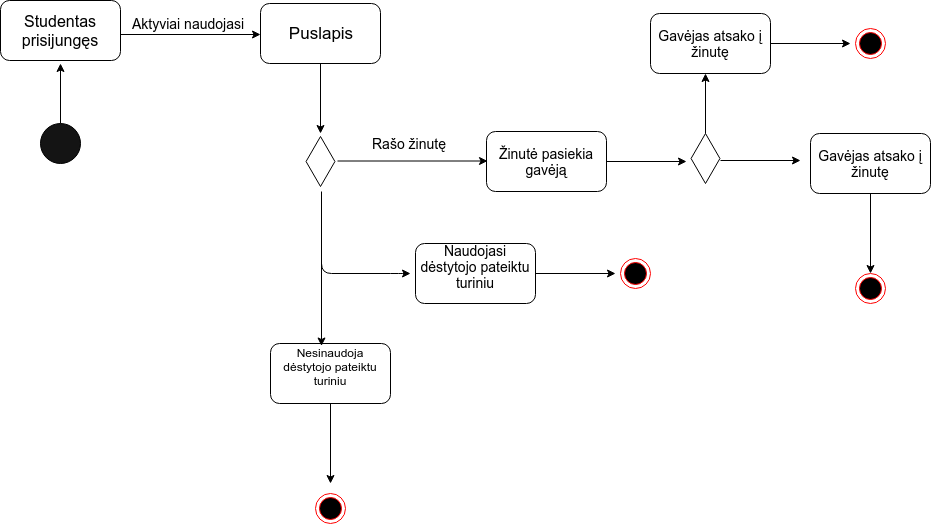
\includegraphics[width=\linewidth]{img/studentas.png}
\caption{Studento UML klasių diagrama}
\label{fig:studentu}
\end{figure}
\ref{fig:studentu} pav. Prisijungęs studentas turi galimybę matyti bendrą turinį. Vėliau gali parašyti žinutę dėstytojui arba naudojasi dėstytojo pateiktu turiniu. Jie tarpusavyje gali komunikuoti socialinio tinklo pagalba, nenaudojant trečiųjų šalių servisų.
\end{document}